\chapter{Literature Review}\label{chap:litrev}

\section{Introduction}\label{sec:litrev:intro}

\textit{Bacillus subtilis} biofilms exhibit an intricate combination of cellular differentiation and paracrine signaling, making them a compelling model for studying bacterial multicellularity.{\footnotesize\cite{Lyons2015}\cite{Lpez2009}} Despite sharing identical genetic material, \textit{Bacillus subtilis} cells within a biofilm demonstrate remarkable heterogeneity in phenotype. This phenomenon is triggered by a set of signaling pathways and gene regulatory networks. {\footnotesize\cite{chai_vlamakis_kolter_2011}\cite{Vlamakis2008}}

In this literature review, we explore the mechanisms behind the self-organization properties of \textit{B. subtilis}. We examine the macroscopic patterns exhibited by \textit{B. subtilis} biofilms and the role of cellular differentiation and cell signaling on these macroscopic behaviors. In \textit{B. subtilis} biofilms, certain cells specialize in producing signaling molecules that induce phenotype switching in other nearby cells. This process is known as paracrine signaling {\footnotesize\cite{Lpez2009}}. Furthermore, specific gene regulatory pathways, such as those involved in surfactin (a signaling molecule which is also a surfactant molecule) production and regulation of matrix production, are examined to gain insights into the differentiation process.
Finally, we will describe the mathematical models developed to simulate the gene regulatory network that controls matrix production. This involves simulating the dynamic cytoplasmic concentrations of SinR, SinI, and SlrR proteins.

\section{\textit{Bacillus subtilis} Biofilms}\label{sec:litrev:theme1}
Bacterial cells usually do not live in isolation; instead, they live and interact in complex communities. They typically flourish in large clusters of cells surrounded by a protective self-secreted extracellular matrix, forming biofilms. Biofilms are ubiquitous and can be found in diverse environments, ranging from dental plaque to water pipelines. Biofilms are, in some ways, similar to multicellular tissues, as they exhibit collective behaviors that greatly enhance the survival and proliferation of bacteria.{\footnotesize\cite{Webb2003}\cite{Lyons2015}} Among the collective behaviors exhibited by biofilms are adhesion and aggregation, which facilitate colony formation; mechanical stability and water retention{\footnotesize\cite{Ido2020}}, ensuring the biofilm's resilience in various environments; and antibiotic resistance{\footnotesize\cite{Mah2012}}, which protects the bacteria within the biofilm from antimicrobial treatments.

Biofilms of \textit{Bacillus subtilis} serve as a good model for exploring emergent behaviors in bacteria. This is primarily due to their well-understood genetic regulatory networks and their frequent use as model organisms. A prominent characteristic of these biofilms is their ability to demonstrate phenotype differentiation in a switch-like manner, as well as the spatiotemporal heterogeneous expression of these diverse phenotypes within the biofilm. {\footnotesize\cite{Lpez2009}\cite{Srinivasan2018}\cite{Vlamakis2013}}

In a study {\footnotesize\cite{Srinivasan2018}}, researchers demonstrated the spatial progression of distinct phenotype activation during the developmental stages of a \textit{Bacillus subtilis} biofilm (see Figure 2.1). The study involved tracking gene expression using gene reporters for motility, matrix production, and sporulation. The findings from this study further strengthen the existing body of evidence, confirming that \textit{Bacillus subtilis} biofilms exhibit dynamic gene expression that is not uniformly distributed, but rather organized in a distinct spatiotemporal manner. These findings suggest a similarity between biofilms and the tissues of more complex multicellular organisms in terms of functional specialization and spatial organization.

\begin{figure}[h]
    \centering
    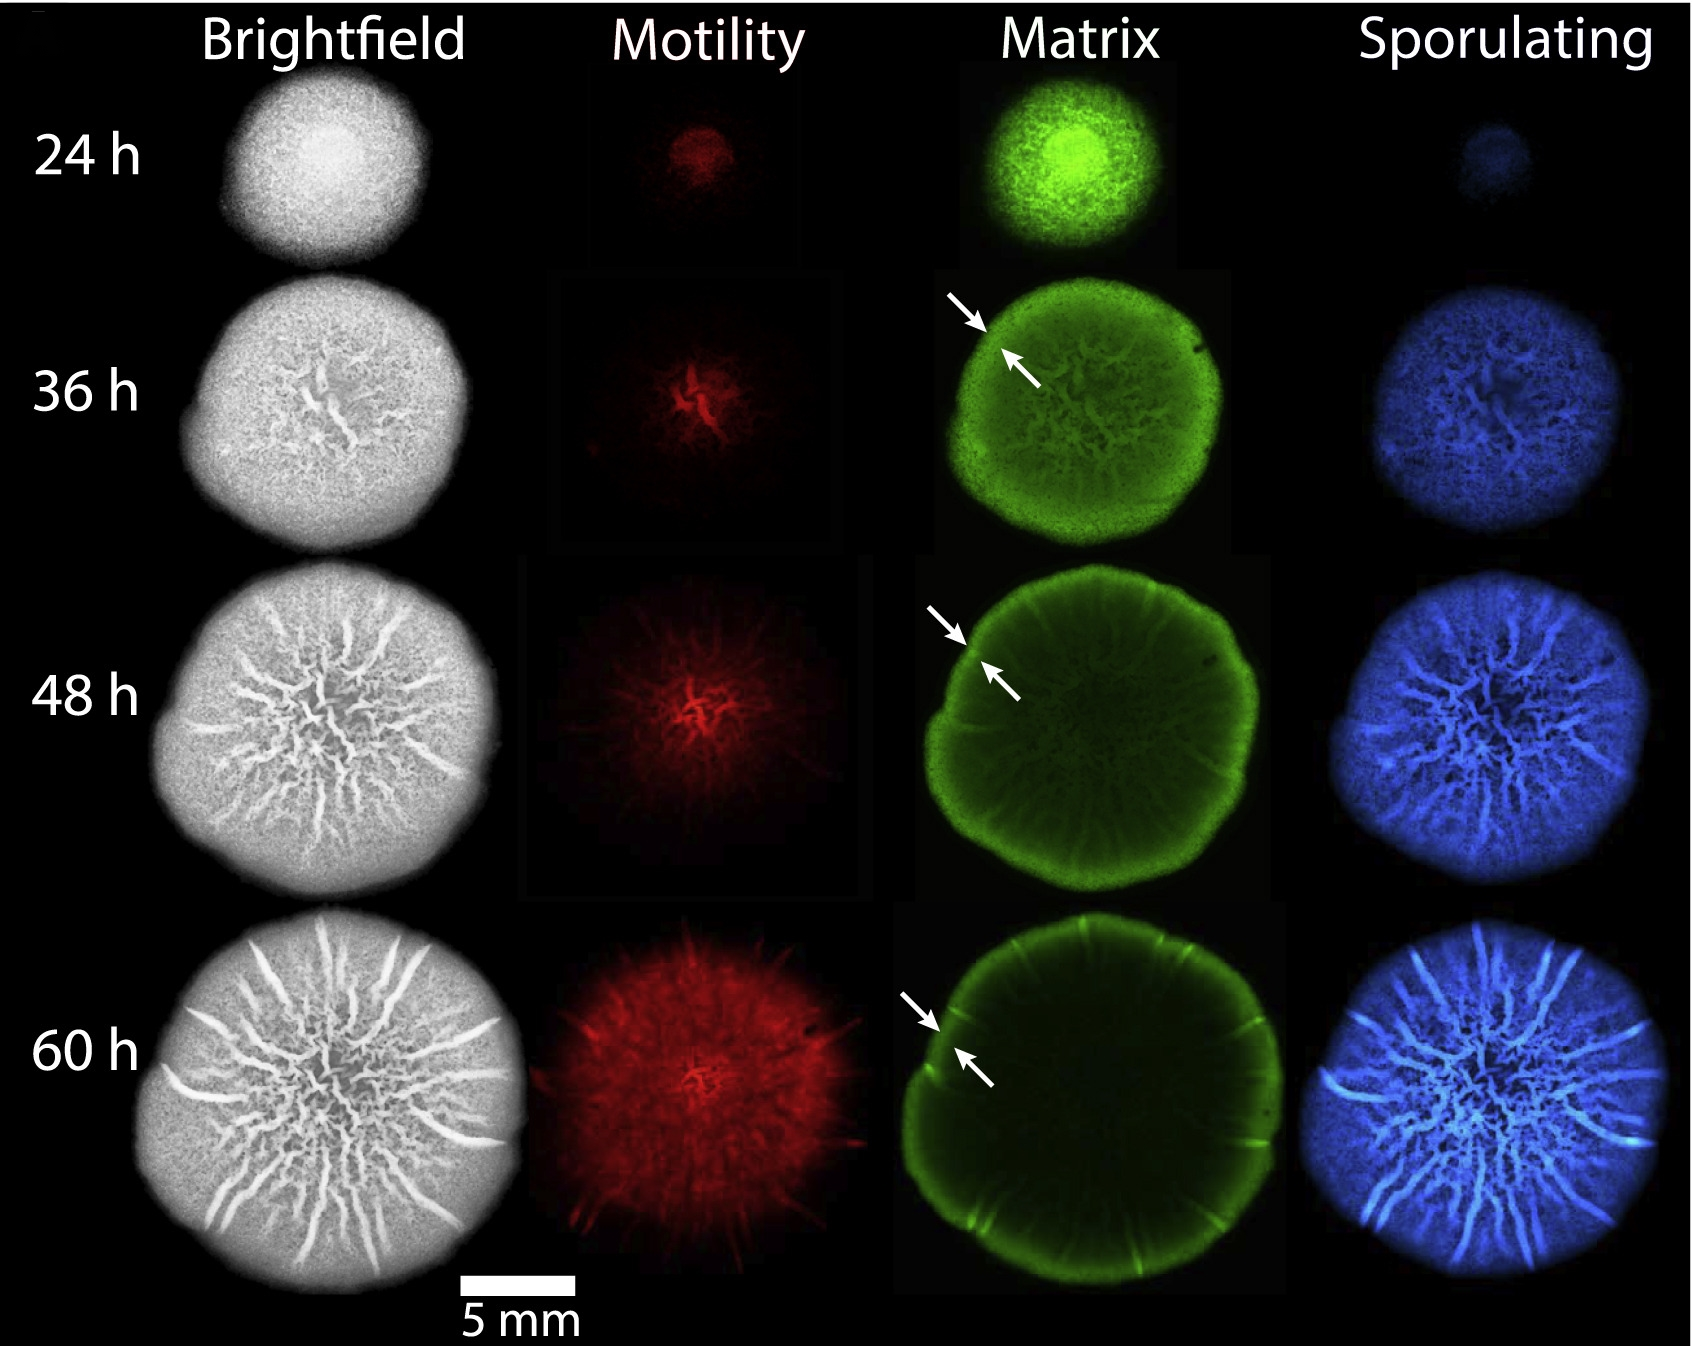
\includegraphics[width=0.8\textwidth]{re}
    \caption{\footnotesize \textbf{Time-lapse of \textit{B. subtilis} biofilm development.} The distinct gene activations are tracked using fluorescent reporters. Activation of genes involved in motility is shown in red, matrix production in green, and sporulation in blue.{\footnotesize\cite{Srinivasan2018}}}


\end{figure}



\section{Paracrine signaling}\label{sec:litrev:theme2}

The observed macroscopic spatial and temporal patterns of gene activation in the \textit{Bacillus subtilis} biofilm suggest a certain level of organization. There is a growing body of evidence suggesting that these patterns are regulated by signaling networks and mechanical interactions between cells, facilitated by signaling molecules that diffuse in the surrounding environment. These communication networks are a common feature of bacterial communities, enabling them to synchronize gene expression. As the density of the cell population increases, these signaling molecules progressively accumulate in the extracellular environment. When reaching a critical concentration, these signaling molecules trigger the coordinated expression of specific genes.{\footnotesize\cite{Arnaouteli2021}}

In many species of bacteria, gene activation and the differentiation of phenotypes are typically regulated by autocrine signaling. Autocrine signaling implies that the cells that produce the signaling molecules are also the same cells that respond to those same signaling molecules. However, in the case of \textit{Bacillus subtilis}, studies suggest that the mechanism of paracrine signaling, rather than autocrine signaling, plays a role in cell differentiation.{\footnotesize\cite{Lpez2009}} This implies that within the biofilm of \textit{B. subtilis}, there is a division of roles among cells. A specific subpopulation specializes in producing a distinct signaling molecule, while another subpopulation responds to this signal. In the case of \textit{Bacillus subtilis}, the ComX pheromone and surfactin are the two most important signaling molecules involved in biofilm formation.{\footnotesize\cite{Chai2011}\cite{Lpez2009}}



\begin{figure}[h]
    \centering
    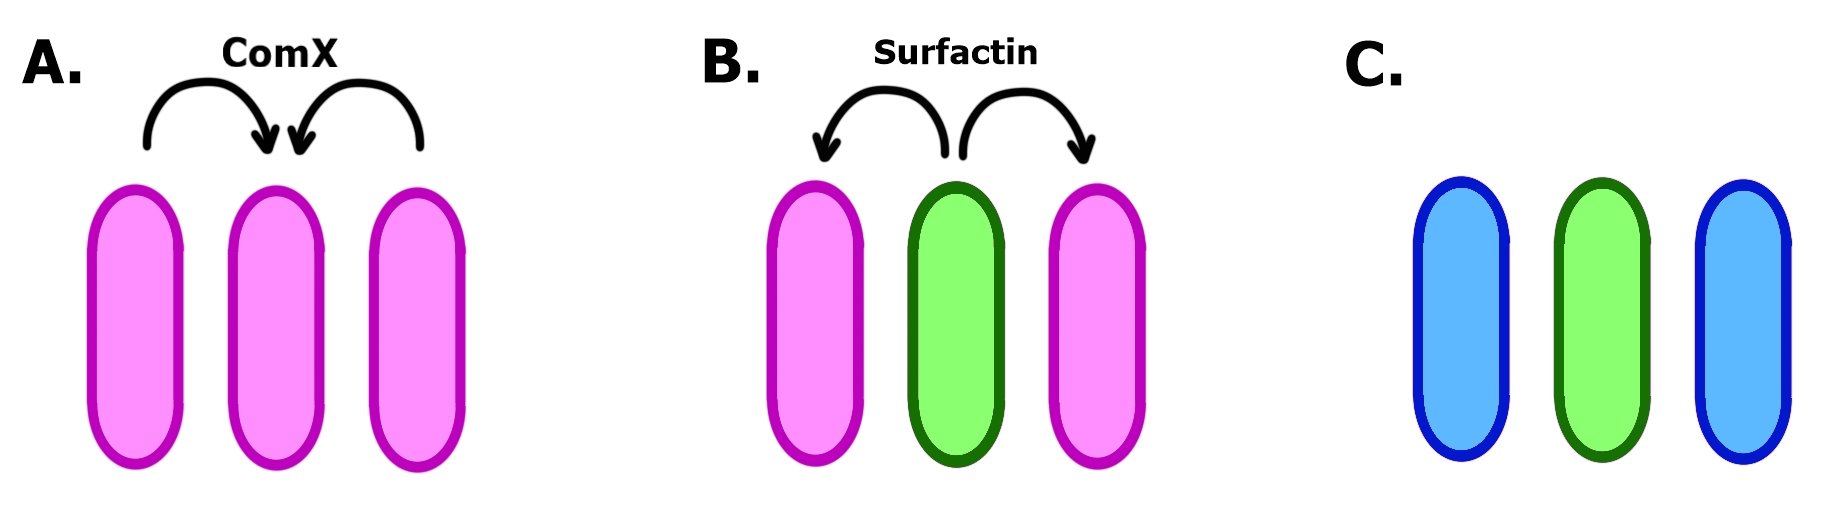
\includegraphics[width=0.8\textwidth]{paracrine}
    \caption{\footnotesize \textbf{Paracrine signaling network in \textit{B. subtilis}} Undifferentiated cells are depicted in pink, surfactin-producing cells are depicted in green, and matrix-producing cells are depicted in blue. A) All undifferentiated cells produce ComX. Some of the undifferentiated cells are particularly sensitive to ComX, which triggers the activation of the surfactin-producing phenotype. B) Surfactin-producing cells secrete surfactin, which affects the neighboring cells. C) Surfactin activates the genes responsible for matrix production in specific, susceptible cells.{\footnotesize\cite{Chai2011}\cite{Lpez2009}}}


\end{figure}
The general overview of the paracrine signaling network in \textit{B. subtilis} is illustrated in Figure 2.2. The ComX molecule is secreted by all bacteria, regardless of their phenotype. As the cell population grows, the concentration of the ComX pheromone accumulates in the extracellular environment until it reaches a higher threshold. Once this threshold is reached, it triggers a subpopulation of nearby bacteria to differentiate into the surfactin-producing phenotype. Then, the subpopulation of bacteria that expresses the surfactin-producing phenotype completely stops growing and reproducing{\footnotesize\cite{Lpez2009}}, and instead begins producing the second signaling molecule: surfactin. Just like ComX, surfactin will begin to accumulate in the environment as the population of surfactin-producing bacteria grows. The high concentration of surfactin in the environment triggers neighboring cells to start producing the extracellular matrix. Interestingly, the cells that produce surfactin are immune to the effects of surfactin. This implies that, as long as a bacterium is expressing the surfactin-producing phenotype, it will not transition into the matrix-producing phenotype. In this sense, the signaling network is a paracrine one.{\footnotesize\cite{Lpez2009}}

Once the bacteria have activated the genes responsible for producing the extracellular matrix, they will develop immunity to the ComX pheromone. This means that the bacteria expressing the matrix-producing phenotype will not switch to the surfactin-producing phenotype. Once again, demonstrating paracrine signaling. The mechanism by which the cell acquires immunity to the ComX pheromone is not fully understood. However, there is evidence suggesting that the extracellular matrix creates a protective layer that inhibits the interaction between ComX and the membrane protein ComP, the protein responsible for sensing ComX.{\footnotesize\cite{Lpez2009}}

\section{Cytoplasmic Gene Regulatory Networks}\label{sec:litrev:theme2}

\subsection{Activation of the surfactin-producing phenotype}\label{sec:litrev:theme2}
The molecular mechanism by which cells switch from one phenotype to another is outlined in Figure 2.3. The ComX pheromone is secreted by all cells and diffuses through the extracellular space. The ComP protein, located in the cell membrane, interacts with the ComX pheromone, which triggers the phosphorylation of the cytoplasmic protein ComA. Upon phosphorylation, ComA is activated and functions as a gene transcription factor for the \textit{srfA} operon. This operon comprises four open reading frames (ORFs) that collectively produce the enzyme surfactin synthetase. Surfactin synthetase is a nonribosomal peptide synthetase, an enzyme that synthesizes peptides such as surfactin without the need for ribosomes. {\footnotesize\cite{Lpez2009}\cite{Rahman2021}}


\begin{figure}[h]
    \centering
    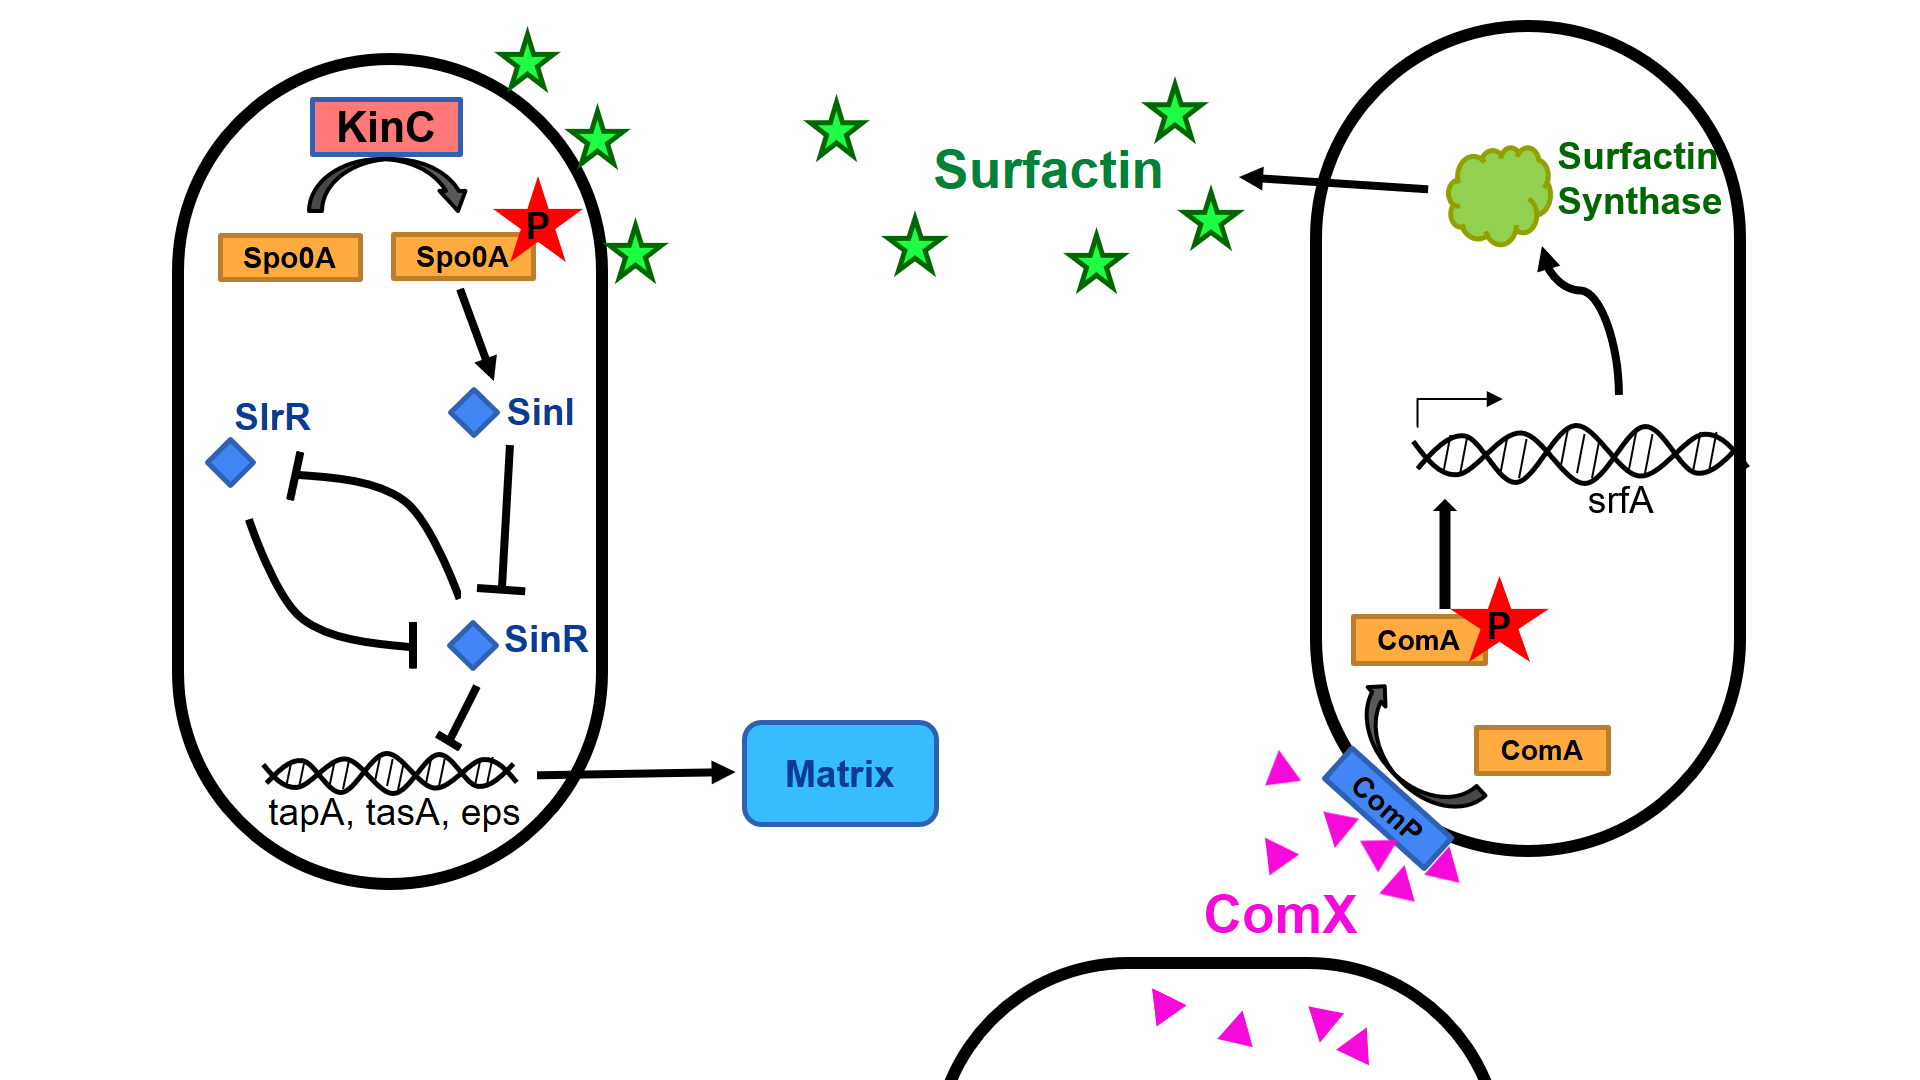
\includegraphics[width=1\textwidth]{Screenshot}
    \caption{\footnotesize \textbf{Extracellular signaling network and cytoplasmatic gene regulatory network} {\footnotesize\cite{Rahman2021}}}



\end{figure}

\subsection{Activation of the Matrix-producing phenotype}\label{sec:litrev:theme2}

Surfactin is known to indirectly activate the expression of genes that produce matrix, although the precise molecular process is not fully understood. It has been suggested that surfactin creates pores in the membrane, leading to the leakage of potassium ions from the cytoplasm to the outside of the cell. This causes the activation of the membrane sensor kinase KinC when potassium levels are low, which then phosphorylates the master gene regulator Spo0A.{\footnotesize\cite{Lpez20091}} However, some studies contradict this exact mechanism.{\footnotesize\cite{Devi2015}}

When Spo0A is activated, it triggers the transcription of the SinI protein. The SinI protein binds to the SinR protein to form a SinI-SinR complex, which effectively titrates SinR, reducing the number of freely available SinR proteins. SinR is a protein that suppresses the transcription of genes related to matrix production. By disabling SinR through the formation of the SinI-SinR complex, the cell can activate the genes responsible for matrix production.{\footnotesize\cite{Chai2011}}

Furthermore, SinR also inhibits the expression of another protein known as SlrR. If SlrR is expressed, it can also suppress SinR by interacting with it to form a SlrR-SinR complex.{\footnotesize\cite{Chai2011}}

\subsection{Mathematical modelling of SlrR-SinI-SinR gene regulatory network}\label{sec:litrev:theme2}
Several authors have formulated systems of differential equations to quantitatively model the biomolecular dynamics involved in the gene regulatory network that controls the expression of the extracellular matrix. The systems of equations describe the changes in the concentration of SinR, SinI, and SlrR proteins in the cytoplasm of individual \textit{Bacillus subtilis} cells over time.{\footnotesize\cite{simon}\cite{Voigt2005}\cite{Newman2013}\cite{Chen2023}\cite{Pedreira2021}\cite{Hallinan2010}}. Having considered the models proposed by these authors, we have decided to adopt a modified version of the model proposed by Dannenberg et al. {\footnotesize\cite{simon}} as the basis for our own model. The model is described by the following system of differential equations:

\begin{align}
\frac{dR}{dt} &= P_{3} - D_{R} R - K_{on(RI)} R I - K_{on(RL)}RL , \label{eq:1} \\
\frac{dI}{dt} &= P_{1}g(R)f(A) - D_{I} I - K_{on(RI)} R I , \label{eq:2} \\
\frac{dL}{dt} &= P_{L}g(R) - D_{L} L - K_{on(RL)} RL, \label{eq:3}
\end{align}

where \(P_3\), \(P_1\), and \(P_L\) represent the maximum production rates of SinR, SinI, and SlrR, respectively. \(R\), \(I\), and \(L\) represent the respective total protein concentrations within a single bacterial cell. \(K_{on(XY)}\) represents the rate constant for the formation of the $(XY)$ complex, while \(D_Z\) encompasses both the dilution rate of component $Z$ caused by cell growth and the degradation rate caused by protein breakdown. The phenomenological activation Hill function \(f(A)\) and the repression Hill function \(g(R)\) are defined as follows:


\begin{align*}
    f(A) &= \left(\frac{(A/K_A)^{n_A}}{1 + (A/K_A)^{n_A}}\right) \\
    g(R) &= \left(\frac{1}{1 + (R/K_R)^{n_R}}\right) \\
\end{align*}  

where $A$ represents the concentration of Spo0A in the cytoplasm. \(K_{A}\) and \(K_R\) represent the binding affinities of Spo0A and SinR, respectively, while \(n_A\) and \(n_R\) represent the cooperativities of the binding.

Equation (\ref{eq:1}) describes the dynamics of the SinR protein concentration in the cell. SinR is produced at a constant rate $P_3$, but its concentration is reduced by a combination of degradation and dilution at a rate $D_R$ due to cell growth. Additionally, the concentration of SinR is affected by its interaction with SinI and SlrR, which form complexes with SinR at rates $K_{on(RI)}$ and $K_{on(RL)}$, respectively, leading to a reduction in free SinR molecules.

Equation (\ref{eq:2}) represents the changes in the concentration of SinI. SinI is produced according to its own maximum production rate $P_1$, which is modulated by the function $g(R)$ that models SinR's repression, and the function $f(A)$ which accounts for activation by Spo0A. Just like SinR, the concentration of SinI is decreased both by degradation and dilution at a rate of $D_I$, and by its binding to SinR, forming the RI complex at a rate of $K_{on(RI)}$.

Lastly, Equation (\ref{eq:3}) represents the dynamics of the SlrR protein concentration. The synthesis of SlrR is again dependant on a production rate ($P_L$), modulated by the function $g(R)$ representing the repressive effect of SinR on SlrR transcription. Similarly, it also considers SlrR's degradation and dilution through the rate $D_L$ and its interaction with SinR, which sequesters SlrR into the RL complex at the rate $K_{on(RL)}$.

The Hill functions in the model represent the regulatory effects of two proteins, Spo0A and SinR, in a phenomenological manner. The activation Hill function \( f(A) \) models the phenomenon in which Spo0A promotes the gene responsible for producing SinI after reaching a critical concentration threshold ($K_A$). This effect exhibits a cooperative nature, meaning Spo0A molecules support each other's binding, resulting in a "switch-like" type of gene activation. On the other hand, the repression Hill function \( g(R) \) describes how SinR inhibits the expression of genes that produce SlrR and SinI. As the concentration of SinR increases above a threshold ($K_R$), the level of repression becomes significant. The Hill functions mathematically represent the biological processes of gene activation and repression in a sigmoidal, threshold-dependent manner.

The system of differential equations just presented is largely similar to the one proposed by Dannenberg et al. {\footnotesize\cite{simon}}. The main difference is that, unlike Dannenberg et al., this thesis will consider the inhibitory effect of SinR on SinI transcription. This inhibitory effect has been proposed and taken into account by other authors {\footnotesize\cite{Voigt2005}\cite{Pedreira2021}\cite{Dundee2022}\cite{Hallinan2010}}

\section{Conclusion}\label{sec:litrev:conclusion}

Drawing from our literature review on \textit{Bacillus subtilis} biofilms and their cellular dynamics, we are set to construct an agent-based model. This model will simulate the complex behaviors of \textit{B. subtilis} cells, integrating the diffusion of extracellular signaling molecules and the gene regulatory networks that control the intracellular concentrations of SinR, SinI, and SlrR. By translating our theoretical insights into a computational framework, we aim to capture the emergent biofilm properties through \textit{in silico} simulation.
